% LaTeX template for Models of Computation assessed coursework
% Most of the required packages are standard and should be provided by most TeX installations
% The exception is mathpartir, which is provided alongside this document

\documentclass[11pt,a4paper]{article}
\usepackage{float}
\usepackage{caption}
\usepackage{subfig}
\usepackage{graphicx}
\usepackage{fullpage}
\usepackage{rotating}
\usepackage{amsmath, amssymb, amsthm}
\usepackage{stmaryrd}
\usepackage{proof}
\usepackage{mathpartir}
\usepackage{tikz}
\usepackage{verbatim}
\usepackage{url}
\usepackage{multicol}
\usepackage{xr-hyper}
\usepackage[title]{appendix}
\usepackage{titling}
\usepackage{amsthm}
\usepackage{amsfonts}
\usepackage{gensymb}
\usepackage{graphicx}
\usepackage[]{mcode}
% Common macros
%Subtitle 
\newcommand{\subtitle}[1]{%
  \posttitle{%
    \par\end{center}
    \begin{center}\large#1\end{center}
    \vskip0.5em}%
    }
% BNF notation
\newcommand{\Gdef}{\mathrel{\mathop{::}}=}
\newcommand{\Gbar}{\mathbin{\ \big|\ }}
\newcommand{\Coloneqq}{\Gdef}

% Big-step arrow
\newcommand{\bigstep}{\mathrel{\Downarrow}}

% Semantic operators are (often) underlined to avoid ambiguity
\newcommand{\semop}[1]{\mathbin{\underline{#1}}}


% Program syntax is set in teletype using the \cmd macro
\newcommand{\cmd}[1]{\texttt{#1}}

% Macros for program constructs
\newcommand{\ifthen}[3]{
  \cmd{if} \; #1 \; \cmd{then} \; #2 \; \cmd{else} \; #3 }
\newcommand{\while}[2]{
  \cmd{while} \; #1 \; \cmd{do} \; #2 }

% \ang{x} typesets x in angled brackets
\newcommand{\ang}[1]{\langle #1 \rangle}

% The following two macros are for typesetting rules and derivations
% Usage: \drule{rule name}{premise1 \\ premise2 \\ premise3 ...}{conclusion}
% The premises will often also be derivations using \drule.
% The difference between \drule and and \Drule is that the space for the rule name
% is not measured with \Drule.  This is useful for typesetting left-most subderivations.
\newcommand{\drule}[3]{\inferrule*[left={#1}]{#2}{#3}}
\newcommand{\Drule}[3]{\inferrule*[Left={#1}]{#2}{#3}}

% For defininitions
\newcommand{\eqdef}{\triangleq}


% WhileDM
\newcommand{\whiledm}{\textsc{WhileDM}}
% Names of types
\newcommand{\tname}[1]{\mathit{#1}}
\newcommand{\exprs}{\tname{Expr}}
\newcommand{\bools}{\tname{Bool}}
\newcommand{\comms}{\tname{Comm}}
\newcommand{\vars}{\tname{Var}}
\newcommand{\nums}{\tname{Num}}
\newcommand{\addrs}{\tname{Addr}}
\newcommand{\vals}{\tname{Val}}
\newcommand{\stor}{\tname{Store}}
\newcommand{\heap}{\tname{Heap}}
\newcommand{\bv}{\tname{BVal}}
\newcommand{\ad}[1]{\ulcorner {#1} \urcorner}
\newcommand{\newp}{\texttt{newpair}}
\newcommand{\fst}[1]{{#1}.\texttt{fst}}
\newcommand{\snd}[1]{{#1}.\texttt{snd}}
\newcommand{\stof}[2]{\texttt{fst} [ {#1} ] \leftarrow {#2}}
\newcommand{\stos}[2]{\texttt{snd} [ {#1} ] \leftarrow {#2}}
\newcommand{\dom}[1]{\mathrm{dom}(#1)}
\newcommand{\bse}{\bigstep_e}
\newcommand{\bsc}{\bigstep_c}
\newcommand{\bsb}{\bigstep_b}
\newcommand{\types}{\tname{Type}}
\newcommand{\typ}{\tau} % Type variable
\newcommand{\tc}{\Gamma} % Type context
\newcommand{\tnat}{\mathsf{nat}}
\newcommand{\tpair}[2]{(#1,#2)}
\newcommand{\hptyp}[3]{#1 \Vdash #2 : #3}
\newcommand{\tcompat}[3]{#1 ; #2 ; #3 \vdash \textsf{\textup{well-typed}}}
\newcommand{\etyp}[3]{#1 \vdash #2 : #3}

\title{ME146 Energy Conversion Principles}
\subtitle{Project 4}
\author{Yeshas Thadimari \& Rhys Williams}
\date{\today}
\begin{document}
\maketitle
\newpage
\section*{Nomenclature}
\begin{enumerate}
\item $\rho$ = air density
\item $w_i$ = magnitude of air relative velocity
\item $v_1$ = far field wind speed
\item $n$ = the number of blades
\item $C_{L,i}$ = lift coefficient of segment i
\item $K_i$ = chord of segment of i 
\item $r_i$ = radius of segment of i 
\item $\omega$ = angular rotation of speed
\item $\delta r$ = length of segment in radial direction 
\item $\eta$ = Efficiency 
\end{enumerate}
\section*{Division of Tasks}
\begin{itemize}
\item Tasks 1 - 4 - Yeshas, Rhys
\item Write up of results - Yeshas, Rhys
\end{itemize}
%-----------------------TASK 1-------------------------------
\section*{Task 1}
For the first task, we had to derive an equation for the work done by the Wind Turbine using the following equations.

\begin{equation}
d\dot{W} = \frac{1}{3} n\rho w(r) v_1 C_L(r) K(r) \omega r dr
\end{equation}
\begin{equation}
w(r) = \sqrt[]{(\frac{2v_1}{3})^2 + \omega^2 r^2}
\end{equation}
\begin{equation}
K(r) = K_H \bigg[1-\sigma \bigg(\frac{r^2 - r_h^2}{R^2 - r_h^2}\bigg) \bigg]
\end{equation}
We substitute $K(r)$ and $\omega(r)$ into the first equation and reorganize it to give the below equation.
where $\hat{r_h} = \frac{r_h}{R}$ and $\lambda = \frac{\omega R}{v_1}$
We can then use the above equation to calculate the power generated from the turbine.
We then have to calculate for the Betz efficiency which is the maximum possible power obtained from the wind turbine. 
\begin{equation}
\dot{W}_{betz} = \frac{16}{27}(\frac{1}{2}\rho v_1^3 \pi (R^2 - rh^2))\
\end{equation}
We can then use the above equation to calculate for Betz efficiency which is given by 
\begin{equation}
\eta_{betz} = \frac{\dot{W}}{\dot{W}_{betz}}
\end{equation}
\subsection*{Derivation of solution}
Making the substitution for K(r) and w(r) into dW initial leads to the following after sole algebraic manipulation.
\begin{equation}
d\dot{W}_{betz} = B[Cr(a^2+r^2)^{\frac{1}{2}}-Dr^3(a^2+r^2)^{\frac{1}{2}}]
\end{equation}
Where a, B, C and D are constants with respect to r with the following definitions.
\begin{equation}
a = \frac{2v_1}{3\omega}
\end{equation}
\begin{equation}
B = \frac{1}{3}n\rho v_1 \omega^2 K_h C_L
\end{equation}
\begin{equation}
C = 1+\frac{\sigma r^2_h}{R^2 - r^2_h}
\end{equation}
\begin{equation}
D = \frac{\sigma}{R^2 - r^2_h}
\end{equation}
We can now integrate with respect to r between the hub radius $r_h$ and the blade radius R to get the total work output.
\begin{equation}
\dot{W}_{betz} = B\int_{r_h}^R [Cr(a^2+r^2)^{\frac{1}{2}}]dr-B\int_{r_h}^R Dr^3(a^2+r^2)^{\frac{1}{2}}dr
\end{equation}
We use the following identity to integrate the 1st integral turn:
\begin{equation}
\int r(a^2+r^2)dr = \frac{1}{3}(r^2 +a^2)^{\frac{3}{2}}
\end{equation}
And a second identity for the second integration term
\begin{equation}
\int r^3(a^2+r^2)dr = (\frac{1}{5}r^2 -\frac{2}{15}a^2)(r^2 +a^2)^\frac{3}{2}
\end{equation}
After preforming the integral and some algebraic manipulation we find the following function for W, note for convenience of righting it has been left in pre evaluated form.
\begin{equation}
\dot{W} = \frac{1}{3} n\rho v^3_1 C_L K_h \lambda^2 \frac{1}{R^2}[\frac{1}{3}(1+\frac{\sigma \hat{r}_h}{1-\hat{r}_h})-(\frac{\sigma}{R^2(1-\hat{r}^2_h)})(\frac{1}{5}r^2-\frac{2}{15}(\frac{2R}{3\lambda})^2)][(\frac{2R}{3\lambda})^2)+r^2]^{\frac{3}{2}}\Big|_{rh}^R
\end{equation}
Now following through and dividing by the betz efficiency
\begin{equation}
\eta_{Betz} = \frac{\frac{9}{8} n C_L K_h \lambda^2 \frac{1}{R^2}[\frac{1}{3}(1+\frac{\sigma \hat{r}_h}{1-\hat{r}_h})-(\frac{\sigma}{R^2(1-\hat{r}^2_h)})(\frac{1}{5}r^2-\frac{2}{15}(\frac{2R}{3\lambda})^2)][(\frac{2R}{3\lambda})^2)+r^2]^{\frac{3}{2}}\Big|_{rh}^R}{\pi R^2(1-\hat{r}^2_h)}
\end{equation}
\section{Task 2}
For task two  part a equations 14 and 15 are evaluated at the following conditions
\begin{align*}
\rho = 1.18 \quad kg/m^3 \\
v_1 = 12 \quad m/s \\
\alpha = 8 \quad Deg \\
C_L = 1.27 \\
n = 3 \\
K_h = 2.7 \quad m \\
\sigma = 0.3 \\
r_h = 3 \quad m \\
R = 35 \quad m \\
\omega = 2 \quad radians/s \\
\end{align*}
Evaluation of 14 and 15 leads to a power output of 2319687.7 W (or 2.3197 MW ) and a Betz efficiency of 1.0051. The fact that the calculation predicts the Betz efficiency will be exceeded shows the limitation of the theory being used to calculate it as it does not take into account the behavior of the airflow downstream or upstream of the turbine were pressure balances will limit the energy output.\\
For part b of the question the setting angle to keep alpha constant was solved for as follows.
\begin{equation}
\eta = \alpha - tan^{-1}(\frac{2Rv_1}{3wRr})
\end{equation}
The plot of which is as follows:

The above shows as would be expected we have to decreases the setting angle with distance, essentially the blade will point straight down relative to the hub at the tip were the circular velocity is highest.
\section*{Task 3}
In task 3 we are tasked with selection of the radius of the turbine and the constant $\sigma$. We decided to put restraints on the selection of R and $\sigma$, firstly R should be reasonable sized, as centripetal force on the blade scales with the length as follows
\begin{eqnarray}
F_c = m R w^2
\end{eqnarray}
The axial load along the blade will increase with length and hence we should not have a excessively long blade. With this in mind we should also try and have a reasonable high $\sigma$ such that the blade is not end heavy. for this reason the values of $\sigma$ are restricted to be greater than zero. A second concern about blade length is the bending of the blade, if we modal the blade as a beam fixed at one end and free at the over and we assume a close to point load at the tip (this is reasonable for proximate calculations as the tip is moving fastest and generating the most lift than over sections of the blade) we can see the bending stiffness is defined as follows.
\begin{equation}
K_{bending} = 3 \frac{E I_z}{(R-rh)^3}
\end{equation}
equation tells us that the bending stiffness and hence tip deflection decreases rapidly ( to the 3rd power) as we increase R, this is of great concern as there will be large efficiency losses if the be blade bends too much.
The method to solve was to specify all variables that are functions of R, those being Kh, rh, Power and efficiency as symbolic functions in matlab and then forcing the system to be solved for a power output of 1.5 KW for a given value of $\sigma$, the script solves for R which produces the required power for a given $\sigma$ and then calculates Power, efficiency and axial loading of the blade.
\begin{figure}[H]
\centering
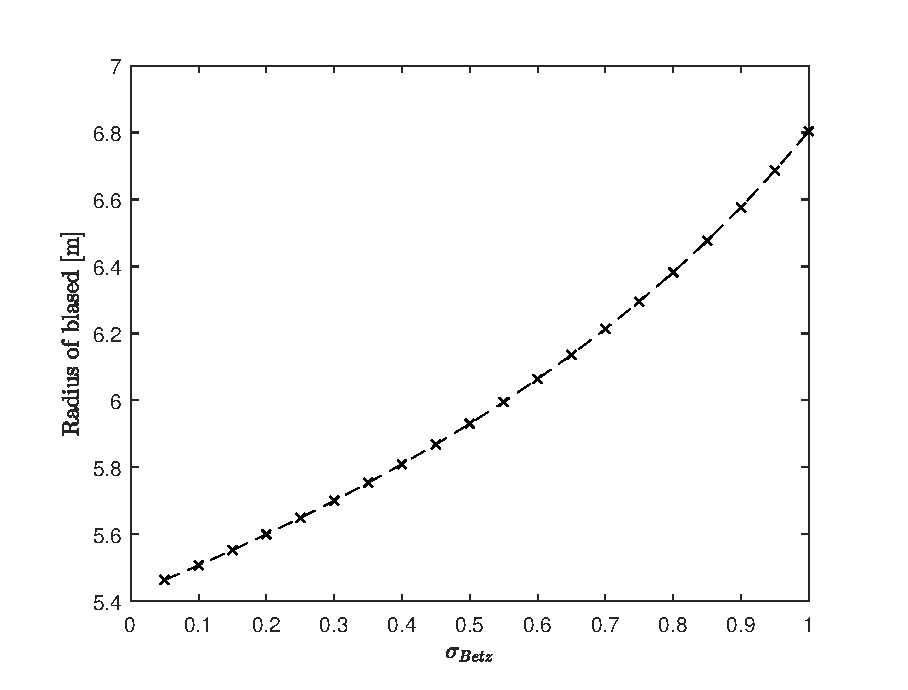
\includegraphics[width=300pts]{RADIUS.eps}
\caption{Radius to produce 1.5 Kw for different $\sigma$ values}
\end{figure}

\begin{figure}[H]
\centering
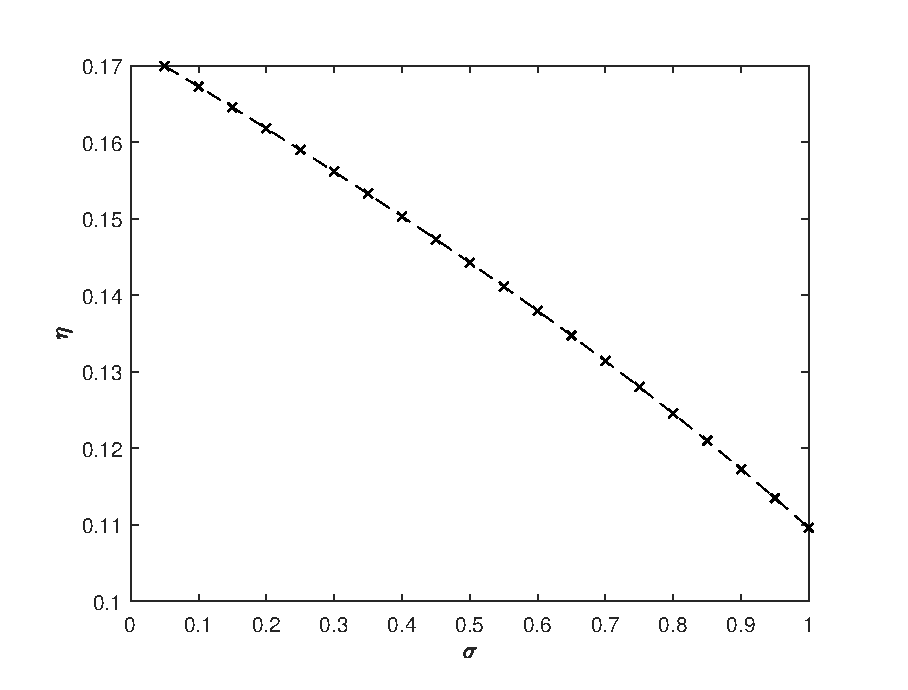
\includegraphics[width=300pts]{BETZ_EFFICIENY.eps}
\caption{Betz efficiency of different blade lengths ( see figure 2) to produce 1.5 Kw for different $\sigma$ values}
\end{figure}

\begin{figure}[H]
\centering
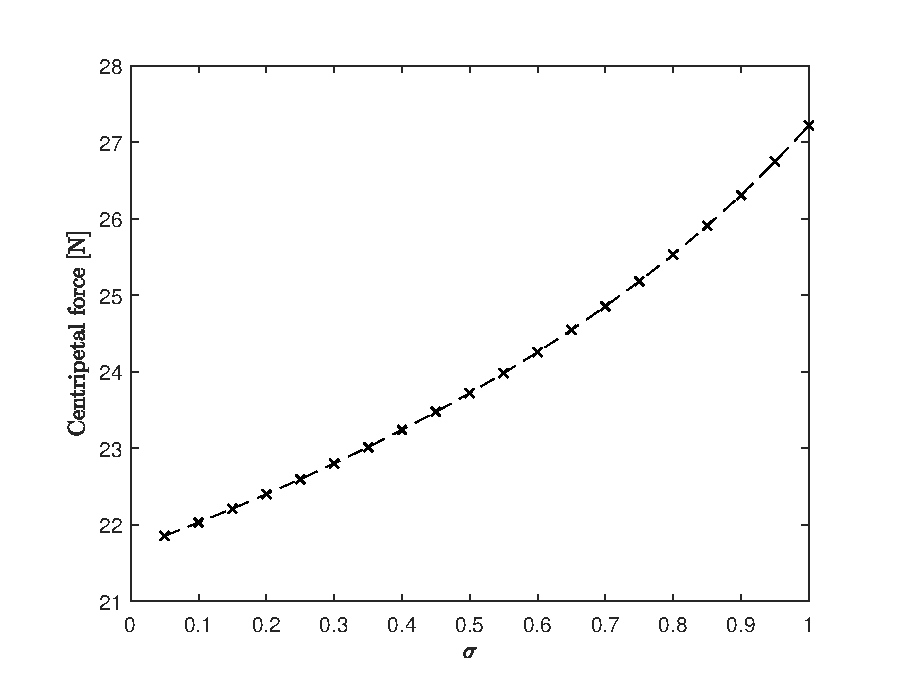
\includegraphics[width=300pts]{LOADING.eps}
\caption{Blade loading axial of different blade lengths ( see figure 2) to produce 1.5 Kw for different $\sigma$ values}
\end{figure}

Picking a sensible value for blade length, a 5.6 m max radius blade would be a good compromise producing high efficiency with low axial loading and a reasonable $\sigma$ such that the blade is not end heavy, this will give a sigma of approximately 0.3 and betz efficiency in the rand of 0.16 (16$\%$). The design choices were also made in context of the max and min wind speed available, although it is unlikely this design will be very effective at low wind speeds it would be structural stable and would not undergo to much bending at high speeds.
\section*{Task 4a \& 4b}
For Task 4a we are simply asked to calculate the delivered current from the turbine of Task 3 if the generator produced a 12V DC. Using $\frac{P}{V} = I$ we get delivered current = 125A. \\ 
For Task 4b we are to use the below equations to calculate the fraction of energy that is extracted from a $H_2-O_2$ fuel cell operating at $I_{cell} = 3.0 A$ for an hour. This is calculated by the below equation
\[\textnormal{Fraction of energy extracted} = \frac{V_{cell,output} I_{cell} t}{V_{cell,input} I_{cell} t}\]
where \[V_{cell,output} = 1.23 - 0.12 - 0.041I_{cell}\] \[V_{cell,input} = 1.23 + 0.12 + 0.041I_{cell}\]
The final value of the fraction extracted is 0.67. 

\begin{appendices}
\section{Task 2}
Matlab Code for Task 2 and Task 1
\begin{lstlisting}
%%% HOUSE KEEPING
clc
clear
%% POWER CALCULATION
rho = 1.18; %DENISTY AIR [kg/m^3]
v1 = 12; %VELOCITY [m/s]
CL = 1.27; %LIFT COEFF
n = 3; %Number of blades
Kh = 2.7; %Chord [m]
gam = 0.3; %Chord turm
rh = 3; %Hub radius [m]
R = 35; %Blad radius [m]
w = 2; % [radians/s]
alpha = 8; %[deg]
%% DEFINE RATIOS
RH = rh/R;
LAM = w*R/v1;
%% CALCULATE POWER
a = (1/3)*n*rho*(v1^3)*CL*Kh*(LAM^2)*(1/(R^2))
POWER = @(r) a*((1/3)*(1+gam*(RH^2)/(1-RH^2))-(gam/((R^2)*(1-RH^2)))*((1/5)*(r^2)-(2/15)*((2*R/(3*LAM))^2)))*(((2*R/(3*LAM))^2+r^2)^(3/2));
POWER_OUT = POWER(R)-POWER(rh)
%% EFFICIENCY CALCULATION
W_betz = (16/27)*(1/2)*rho*(v1^3)*pi*(R^2 - rh^2)
ETA = POWER_OUT/(W_betz)
%% PLOT SETING ANGLE
eta_deg = @(r) ((alpha/180)*(pi) - atan(2*R/(3*(w*R/v1)*r)))*180/pi;
fplot(eta_deg,[rh R])
xlabel('r [m]','Interpreter','latex')
ylabel('$\xi$ [Deg]','Interpreter','latex')

\end{lstlisting}
\section{Task 3}
Matlab Code for Task 3 
\begin{lstlisting}
%%%%% TASK 3 OF FINAL PROJECT | RHYS WILLIAMS %%%
%% HOUSE KEEPING
clc
clear
%% POWER CALCULATION
rho = 1.18; %DENISTY AIR [kg/m^3]
v1 = 6.5; %VELOCITY [m/s]
CL = 1.27; %LIFT COEFF
n = 4; %Number of blades
w = 2; % [radians/s]
alpha = 8; %[deg]
for i = 1:20
    gam = (0.01*i)*5; % itiraye the value of gamma
    G(i) = gam; % store gamme for later plotting
    Kh = @(R) 0.085*R; % calcualte te value for Kh as a function of R
    rh =@(R) 0.1*R  ; % calcualte hub radiuas as a funtion of R
    %% DEFINE RATIOS
    RH = @(R) rh(R)/R;
    LAM = @(R) w*R/v1;
    %% CALCULATE POWER
    a = @(R) (1/3)*n*rho*(v1^3)*CL*Kh(R)*(LAM(R)^2)*(1/(R^2)); % constant outisde of the intigrand solution turm
    POWER = @(r,R) a(R)*((1/3)*(1+gam*(RH(R)^2)/(1-RH(R)^2))-(gam/((R^2)*(1-RH(R)^2)))*((1/5)*(r^2)-(2/15)*((2*R/(3*LAM(R)))^2)))*(((2*R/(3*LAM(R)))^2+r^2)^(3/2));
    POWER_OUT =  @(R) POWER(R,R)-POWER(rh(R),R);
    R_SOLVE(i) = double(solve(@(R) POWER(R,R)-POWER(rh(R),R)==1500));    
    %% EFFICIENCY CALCULATION
    W_betz = @(R) (16/27)*(1/2)*rho*(v1^3)*pi*(R*R - rh(R)*rh(R));
    if R_SOLVE(i)<=0
        break
    end
    ETA = @(R) POWER_OUT(R)/(W_betz(R)-W_betz(rh(R)));
   %% CALCULATE EFFICIENCY FOR THIS SOLVE FOR SIGMA AND R 
    ETAR(i) = ETA(R_SOLVE(i));
    %% LOADING ON BEAM CENTRIFUGALY
    FORCE(i) = 4*R_SOLVE(i);
end
plot(G,ETAR,'--kx'); 
xlabel('$\sigma$','Interpreter','latex')
ylabel('$\eta$','Interpreter','latex')
figure
plot(G,R_SOLVE,'--kx'); 
xlabel('$\sigma_{Betz}$','Interpreter','latex')
ylabel('Radius of blased [m]','Interpreter','latex')
figure
plot(G,FORCE,'--kx'); 
xlabel('$\sigma$','Interpreter','latex')
ylabel('Centripetal force [N]','Interpreter','latex')
\end{lstlisting}
\end{appendices}

\end{document}